%   Copyright 2012 Comet Engineering, Patrick Haring & Christian Bürgi
%
%   Licensed under the Apache License, Version 2.0 (the "License");
%   you may not use this file except in compliance with the License.
%   You may obtain a copy of the License at
%
%       http://www.apache.org/licenses/LICENSE-2.0
%
%   Unless required by applicable law or agreed to in writing, software
%   distributed under the License is distributed on an "AS IS" BASIS,
%   WITHOUT WARRANTIES OR CONDITIONS OF ANY KIND, either express or implied.
%   See the License for the specific language governing permissions and
%   limitations under the License.

\documentclass[fontsize=12pt,
               paper=a4,
               twoside=false,
               parskip=half,
               ]{scrartcl}

% Load the packages
%   Copyright 2012 Comet Engineering, Patrick Haring & Christian Bürgi
%
%   Licensed under the Apache License, Version 2.0 (the "License");
%   you may not use this file except in compliance with the License.
%   You may obtain a copy of the License at
%
%       http://www.apache.org/licenses/LICENSE-2.0
%
%   Unless required by applicable law or agreed to in writing, software
%   distributed under the License is distributed on an "AS IS" BASIS,
%   WITHOUT WARRANTIES OR CONDITIONS OF ANY KIND, either express or implied.
%   See the License for the specific language governing permissions and
%   limitations under the License.

% Packages Template
% =================
% 
% Contains packages used for project documentation
% 
% @author burgc5
% 
% To use this simply enter: %   Copyright 2012 Comet Engineering, Patrick Haring & Christian Bürgi
%
%   Licensed under the Apache License, Version 2.0 (the "License");
%   you may not use this file except in compliance with the License.
%   You may obtain a copy of the License at
%
%       http://www.apache.org/licenses/LICENSE-2.0
%
%   Unless required by applicable law or agreed to in writing, software
%   distributed under the License is distributed on an "AS IS" BASIS,
%   WITHOUT WARRANTIES OR CONDITIONS OF ANY KIND, either express or implied.
%   See the License for the specific language governing permissions and
%   limitations under the License.

% Packages Template
% =================
% 
% Contains packages used for project documentation
% 
% @author burgc5
% 
% To use this simply enter: %   Copyright 2012 Comet Engineering, Patrick Haring & Christian Bürgi
%
%   Licensed under the Apache License, Version 2.0 (the "License");
%   you may not use this file except in compliance with the License.
%   You may obtain a copy of the License at
%
%       http://www.apache.org/licenses/LICENSE-2.0
%
%   Unless required by applicable law or agreed to in writing, software
%   distributed under the License is distributed on an "AS IS" BASIS,
%   WITHOUT WARRANTIES OR CONDITIONS OF ANY KIND, either express or implied.
%   See the License for the specific language governing permissions and
%   limitations under the License.

% Packages Template
% =================
% 
% Contains packages used for project documentation
% 
% @author burgc5
% 
% To use this simply enter: \input{./packages.tex}

\usepackage[utf8]{inputenc}
\usepackage[T1]{fontenc}

% Set font to latin modern
\usepackage{lmodern}

\usepackage[pdftex]{graphicx}
\usepackage{epstopdf}

% Create links in pdf documents
\usepackage[colorlinks,pdfpagelabels,pdfstartview=FitH,bookmarksopen=true,bookmarksnumbered=true,linkcolor=black,plainpages=false,hypertexnames=false,citecolor=black] {hyperref}
\hypersetup{
    colorlinks,%
    citecolor=black,%
    filecolor=black,%
    linkcolor=black,%
    urlcolor=black
}
\urlstyle{same}

% Use \enquote{} to create quotation marks
\usepackage{csquotes}

% Create professional tables with booktabs
% @see http://en.wikibooks.org/wiki/LaTeX/Tables#Professional_tables
\usepackage{booktabs}

% Customizable enumerates/itemizes
\usepackage{enumitem}

% git meta information
\usepackage{gitinfo}


\usepackage[utf8]{inputenc}
\usepackage[T1]{fontenc}

% Set font to latin modern
\usepackage{lmodern}

\usepackage[pdftex]{graphicx}
\usepackage{epstopdf}

% Create links in pdf documents
\usepackage[colorlinks,pdfpagelabels,pdfstartview=FitH,bookmarksopen=true,bookmarksnumbered=true,linkcolor=black,plainpages=false,hypertexnames=false,citecolor=black] {hyperref}
\hypersetup{
    colorlinks,%
    citecolor=black,%
    filecolor=black,%
    linkcolor=black,%
    urlcolor=black
}
\urlstyle{same}

% Use \enquote{} to create quotation marks
\usepackage{csquotes}

% Create professional tables with booktabs
% @see http://en.wikibooks.org/wiki/LaTeX/Tables#Professional_tables
\usepackage{booktabs}

% Customizable enumerates/itemizes
\usepackage{enumitem}

% git meta information
\usepackage{gitinfo}


\usepackage[utf8]{inputenc}
\usepackage[T1]{fontenc}

% Set font to latin modern
\usepackage{lmodern}

\usepackage[pdftex]{graphicx}
\usepackage{epstopdf}

% Create links in pdf documents
\usepackage[colorlinks,pdfpagelabels,pdfstartview=FitH,bookmarksopen=true,bookmarksnumbered=true,linkcolor=black,plainpages=false,hypertexnames=false,citecolor=black] {hyperref}
\hypersetup{
    colorlinks,%
    citecolor=black,%
    filecolor=black,%
    linkcolor=black,%
    urlcolor=black
}
\urlstyle{same}

% Use \enquote{} to create quotation marks
\usepackage{csquotes}

% Create professional tables with booktabs
% @see http://en.wikibooks.org/wiki/LaTeX/Tables#Professional_tables
\usepackage{booktabs}

% Customizable enumerates/itemizes
\usepackage{enumitem}

% git meta information
\usepackage{gitinfo}


\begin{document}

% Document title for title.tex
\newcommand{\doctitle}{Glossary}
% Titlepage Template
% ==================
% 
% @author burgc5
% 
% To use this simply enter: % Titlepage Template
% ==================
% 
% @author burgc5
% 
% To use this simply enter: % Titlepage Template
% ==================
% 
% @author burgc5
% 
% To use this simply enter: \input{./title.tex}
% 
% You have to define the commands '\doctitle' and '\docrevision' to give the 
% document a title and a revision on its titlepage.
% Do this with the following command:
% \newcommand{\doctitle}{Document title goes here}
%
% SVN:
% ----
% You also have to define the variables:
% \SVN $Date$
% \SVN $Revision$
%
% As executing the following command on the file:
% > svn propset svn:keywords "Date Revision" filename.tex
% 
% This titlepage needs:
% \usepackage[pdftex]{graphicx}
% \usepackage{svn}
%

\begin{titlepage}

\begin{center}

% Team-logo
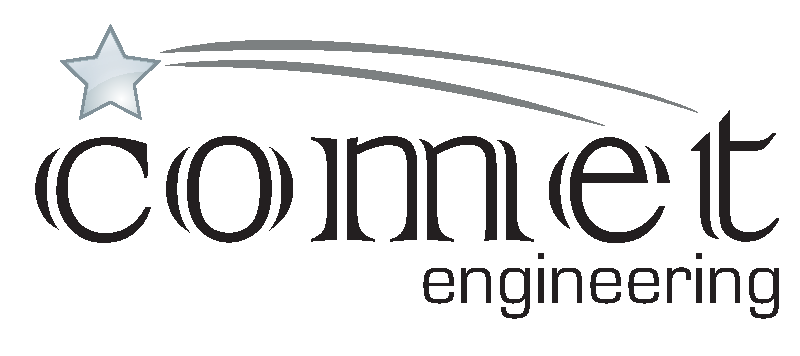
\includegraphics[width=0.35\textwidth]{./comet-logo.eps}\\[2.5cm]    

% Project title
\textsc{\Large Comet Pinball}\\[2cm]

% Document title
{ \huge \bfseries \doctitle{}}\\[3cm]

% Members/Client
\begin{minipage}{0.45\textwidth}
\begin{flushleft} \large
\emph{Team Members:}\\
Patrick \textsc{Haring}\\
Christian \textsc{Bürgi}
\end{flushleft}
\end{minipage}
\begin{minipage}{0.45\textwidth}
\begin{flushright} \large
\emph{Client:} \\
Jean-Pierre \textsc{Caillot}\\
~
\end{flushright}
\end{minipage}

\vfill

{\large 
Revision hash: \gitAbbrevHash \\[0.2cm]
Commit time: \gitCommitterIsoDate \\[0.2cm]
{\footnotesize \itshape \url{https://github.com/boskoop/comet-pinball/}}}

\end{center}

\end{titlepage}
% 
% You have to define the commands '\doctitle' and '\docrevision' to give the 
% document a title and a revision on its titlepage.
% Do this with the following command:
% \newcommand{\doctitle}{Document title goes here}
%
% SVN:
% ----
% You also have to define the variables:
% \SVN $Date$
% \SVN $Revision$
%
% As executing the following command on the file:
% > svn propset svn:keywords "Date Revision" filename.tex
% 
% This titlepage needs:
% \usepackage[pdftex]{graphicx}
% \usepackage{svn}
%

\begin{titlepage}

\begin{center}

% Team-logo
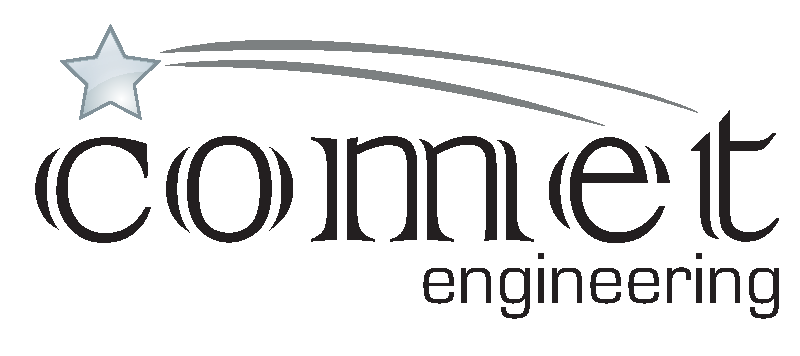
\includegraphics[width=0.35\textwidth]{./comet-logo.eps}\\[2.5cm]    

% Project title
\textsc{\Large Comet Pinball}\\[2cm]

% Document title
{ \huge \bfseries \doctitle{}}\\[3cm]

% Members/Client
\begin{minipage}{0.45\textwidth}
\begin{flushleft} \large
\emph{Team Members:}\\
Patrick \textsc{Haring}\\
Christian \textsc{Bürgi}
\end{flushleft}
\end{minipage}
\begin{minipage}{0.45\textwidth}
\begin{flushright} \large
\emph{Client:} \\
Jean-Pierre \textsc{Caillot}\\
~
\end{flushright}
\end{minipage}

\vfill

{\large 
Revision hash: \gitAbbrevHash \\[0.2cm]
Commit time: \gitCommitterIsoDate \\[0.2cm]
{\footnotesize \itshape \url{https://github.com/boskoop/comet-pinball/}}}

\end{center}

\end{titlepage}
% 
% You have to define the commands '\doctitle' and '\docrevision' to give the 
% document a title and a revision on its titlepage.
% Do this with the following command:
% \newcommand{\doctitle}{Document title goes here}
%
% SVN:
% ----
% You also have to define the variables:
% \SVN $Date$
% \SVN $Revision$
%
% As executing the following command on the file:
% > svn propset svn:keywords "Date Revision" filename.tex
% 
% This titlepage needs:
% \usepackage[pdftex]{graphicx}
% \usepackage{svn}
%

\begin{titlepage}

\begin{center}

% Team-logo
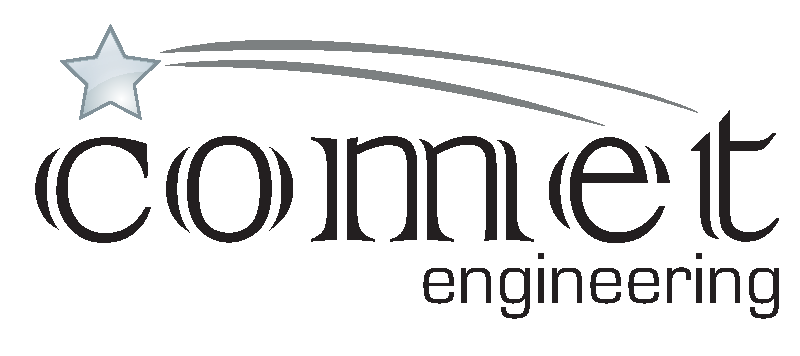
\includegraphics[width=0.35\textwidth]{./comet-logo.eps}\\[2.5cm]    

% Project title
\textsc{\Large Comet Pinball}\\[2cm]

% Document title
{ \huge \bfseries \doctitle{}}\\[3cm]

% Members/Client
\begin{minipage}{0.45\textwidth}
\begin{flushleft} \large
\emph{Team Members:}\\
Patrick \textsc{Haring}\\
Christian \textsc{Bürgi}
\end{flushleft}
\end{minipage}
\begin{minipage}{0.45\textwidth}
\begin{flushright} \large
\emph{Client:} \\
Jean-Pierre \textsc{Caillot}\\
~
\end{flushright}
\end{minipage}

\vfill

{\large 
Revision hash: \gitAbbrevHash \\[0.2cm]
Commit time: \gitCommitterIsoDate \\[0.2cm]
{\footnotesize \itshape \url{https://github.com/boskoop/comet-pinball/}}}

\end{center}

\end{titlepage}

\section*{Glossary}

\subsection*{General terms}

% LaTeX does not support sorting of descriptions. Make sure to insert glossary
% items at the correct position (alphabethically sorted).
\begin{description}

\item[Game]\hfill \\
A game starts when a player launches a ball onto the playfield. It ends when the last ball leaves the playfield (the player can score extra balls which are brought simultaneously onto the playfield). A \emph{simulation} consists normally out of multiple games.

\item[Gameover]\hfill \\
The player is gameover, if there are no more games left at the moment a game ends. Thereby the \emph{simulation} ends and the score is registered.

\item[Highscore]\hfill \\
The highscore is a list which registers the best simulation scores. It is updated if a simulation ends. It has e specific size, if there are more registered scores than available places on the hightscore, the lowest score is dropped.

\item[Pinball machine] \hfill \\
A machine which allows to play pinball. It consists above all out of a playfield and input handles for manipulating the ball.

\item[Score]\hfill \\
Events in a game (e.g. ball hitting a target) are rewarded with points. These are added up to the simulation's score. It is constantly displayed to the player during a game. At the end of a simulation, the score is registered and entered (if high enough) into the highscore.

\item[Simulation] \hfill \\
A simulation includes everything from when a player throws in the first ball until he is \emph{gameover}. Every simulation includes a number of games which the player can play.

\end{description}

\subsection*{Control handles}

% LaTeX does not support sorting of descriptions. Make sure to insert glossary
% items at the correct position (alphabethically sorted).
\begin{description}

\item[Flipper button] \hfill \\
A pinball machine has two buttons for controlling the flippers on the playfield, one on the left and one on the right. Each one of it controls the flipper(s) on its side of the playfield. The buttons are only activated, if there is a ball in play.

\item[Plunger] \hfill \\
The plunger is a spring-loaded rod with a small handle, used to propel the ball into the playfield. The player can control the amount of force used for launching by pulling the plunger a certain distance (thus changing the spring compression).

\end{description}

\subsection*{Playfield elements}

% LaTeX does not support sorting of descriptions. Make sure to insert glossary
% items at the correct position (alphabethically sorted).
\begin{description}

\item[Bumper] \hfill \\
Round knobs that, when hit, will actively push the ball away. % by wikipedia
The player will be rewarded with points when the ball hits a bumper.

\item[Flipper] \hfill \\
Every pinball field has at least two flippers, which are levers controlled by the player. They are used for redirecting the ball up the playfield and therefor preventing it from leaving through the drain.

\item[Hole] \hfill \\
Holes on the playfield into which the player tries to direct the ball. Doing so will reward the player with points. Afterwards the ball is kicked out to bring the ball back into the game.

\item[Ramp] \hfill \\
As the name implies, ramps are inclined planes, with a gentle enough slope that the ball may travel along it. The player attempts to direct the ball with enough force to make it to the top of the ramp and down the other side. If the player succeeds, a "ramp shot" has been made. % by wikipedia

\item[Rollover] \hfill \\
Rollovers are targets which are activated, when a ball rolls over them.

\item[Slingshot] \hfill \\
Slingshots are rubber pads which propel the ball away upon impact, like bumpers, but are usually a horizontal side of a wall. Every recent pinball machine includes slingshots to the upper left and upper right of the lowest set of flippers. % by wikipedia

\item[Stopper] \hfill \\
Also called a \emph{magic post}, this is a small pole most often found centered between and just below the lowest set of flippers. When activated (typically by hitting a specific target or targets), the pole ascends from inside the table, blocking the area between the flippers for a limited time, making it more difficult to drain and lose the ball. After time expires, it returns to its resting place just below the playfield. % by wikipedia

\item[Switch] \hfill \\
A switch is an area that is blocked off after the ball passes through it once. An example of this is the initial firing lane: as a ball passes through the firing lane, it hits a switch and cannot reenter that chute. % by wikipedia

\item[Target] \hfill \\
Targets record when a ball strikes them. The player will be rewarded with points when hitting a target.

\end{description}

\end{document}
